\documentclass{article}

\title{Advent of Code 2024}
\subtitle{Reflection on puzzles and OCaml.}
\date{2025-01-02}
\modified{2025-01-02}

\keyword{programming}
\keyword{puzzles}
\keyword{ocaml}

\begin{document}

\section*

\begin{figure}
  \marginnote{mn-aoc-screen}{Screenshot of the 2024 event page.}
  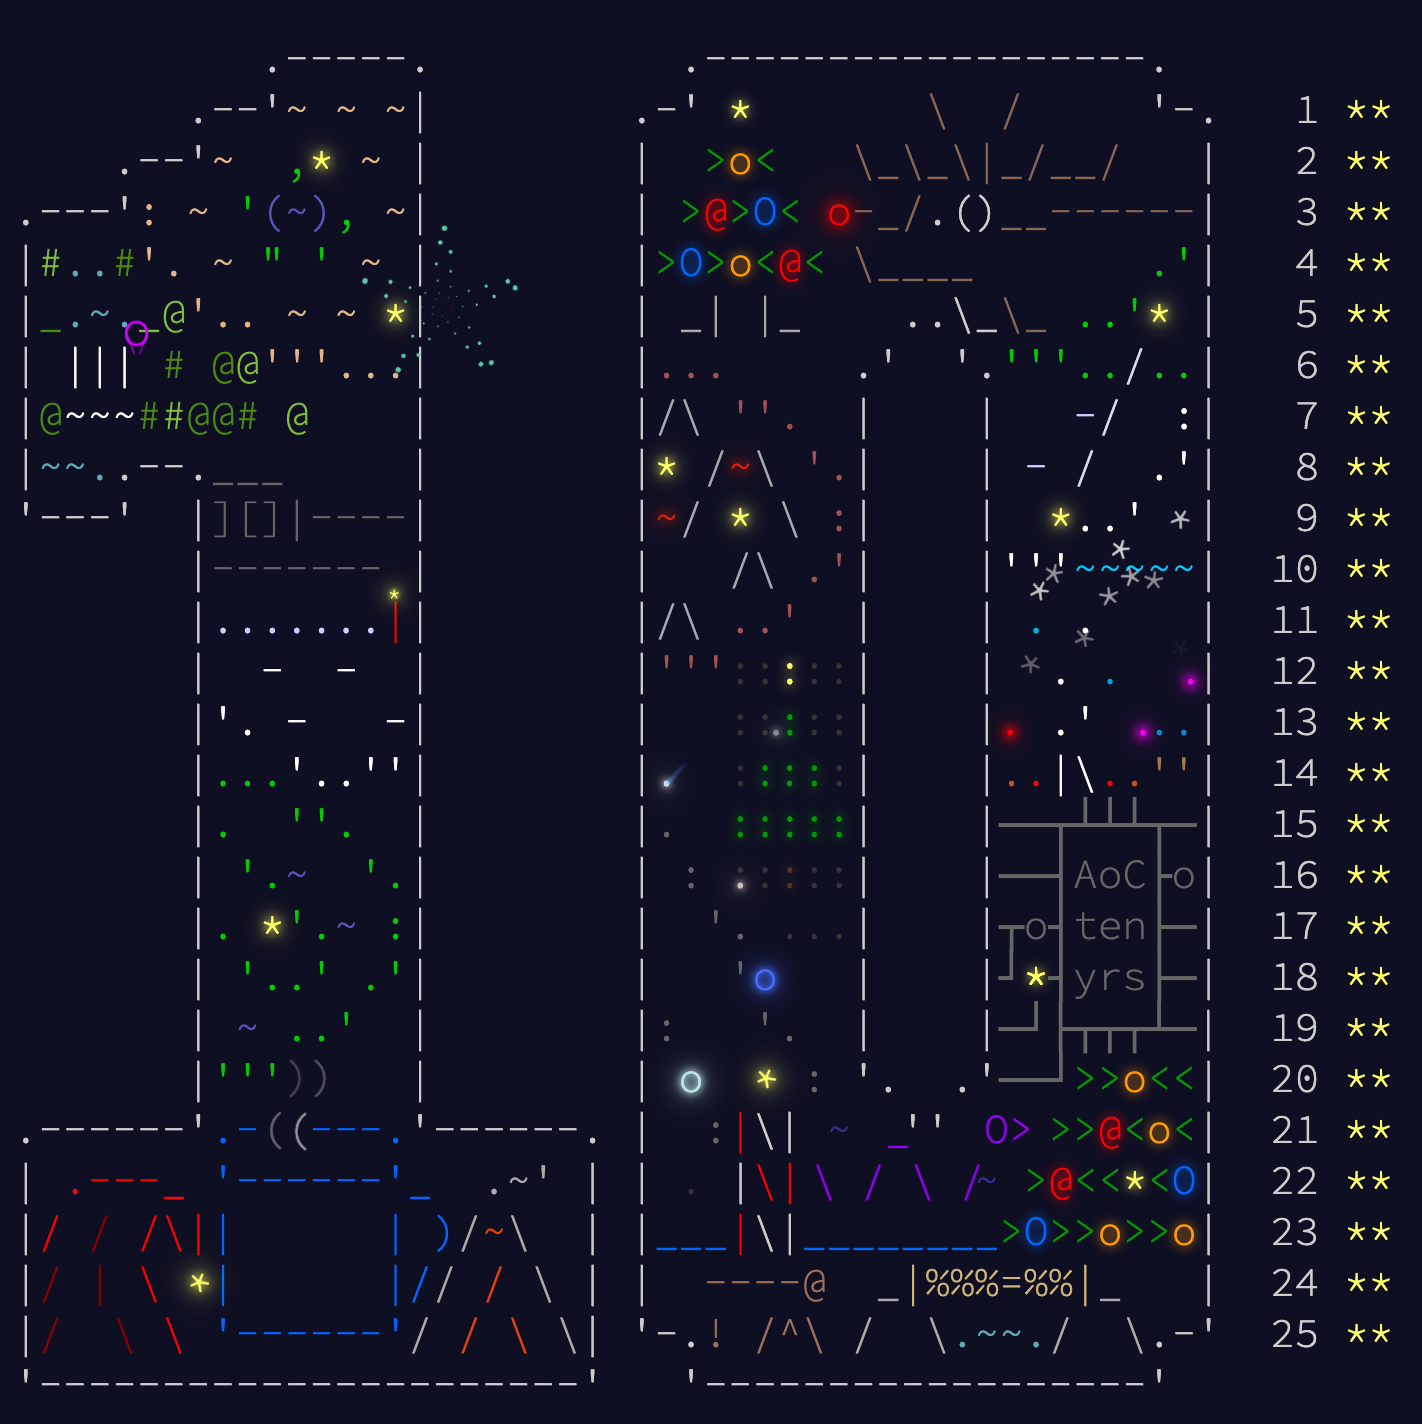
\includegraphics{/images/35-aoc-screen.png}
\end{figure}

Advent of Code (AoC) 2024 was my first advent of code.
I chose OCaml to solve this year's puzzles.
I used it before on online judge websites (e.g., \href{https://www.hackerrank.com/}{Hackerrank}) and felt productive with the language.

This article describes solutions to the puzzles I enjoyed the most and reflects on OCaml's pros and cons in the AoC context.

\section{puzzles}{Puzzles}

Most AoC puzzles were fun, but some stirred more profound experiences: aesthetic appreciation, struggle, and the exhilaration of finally cracking the code.
This section describes solutions to three puzzles.

\subsection{hoof-it}{Day 10: Hoof It}

The \href{https://adventofcode.com/2024/day/10}{Hoof It} puzzle asks you to count particular paths on a grid.
The grid elements are integers from zero to nine representing heights; a path exists between two neighboring cells if their heights differ by one.
The first part asks you to count unique combinations of zeros and nines between which a path exists.
The second part asks you to count the number of \emph{distinct} paths between ones and nines.

This puzzle wasn't hard, but it's an interesting example of dynamic programming on a graph.
I could express both parts with a single algorithm parameterized over the monoid type accumulating answers for each cell.
In the first part, the monoid is the set of all the nines reachable from a cell with the set union operation.
In the second, it's the additive monoid of integers representing the number of distinct paths leading to nines.

This question is perfect for demonstrating OCaml's \href{https://dev.realworldocaml.org/first-class-modules.html}{first-class modules},

The \code{DpMonoid} module signature describes the interface for types we’ll use for dynamic programming.

\begin{code}[ocaml]
module type DpMonoid = sig
  type t
  \emph{(** The neutral element of the monoid. *)}
  val identity : t
  \emph{(** Combine two monoidal values. *)}
  val append : t -> t -> t
  \emph{(** Wrap a "nine" on the grid at the specified location into a monoidal value. *)}
  val inject : int -> int -> t
  \emph{(** Convert a monoidal value to a path score. *)}
  val project : t -> int
end
\end{code}


The \code{count} function implements the dynamic programming driver.
It builds a matrix of monoidal values,
accumulates these values along valid paths starting from nines,
and counts path scores at zero heights.

\begin{code}[ocaml]
let count (map : int array array) (module M : DpMonoid) : int =
  let n, m = Array.length map, Array.length map.(0) in
  let dp = Array.make_matrix n m M.identity in
  let each f = for i = 0 to n-1 do for j = 0 to m-1 do f i j done done in
  each (fun i j -> if map.(i).(j) == 9 then dp.(i).(j) <- M.inject i j);
  for d = 8 downto 0 do
    each (fun i j -> if map.(i).(j) == d then
                       Array.iter (fun (dx, dy) ->
                           let x, y = i + dx, j + dy in
                           if x >= 0 && x < n && y >= 0 && y < n && map.(x).(y) == d+1 then
                             dp.(i).(j) <- M.append dp.(i).(j) dp.(x).(y);
                         ) [|(1, 0); (-1, 0); (0, 1); (0, -1)|]
      )
  done;
  let total = ref 0 in
  each (fun i j -> if map.(i).(j) == 0 then total := !total + M.project dp.(i).(j));
  !total
\end{code}


The entry point calls the \code{count} function twice with different monoids:
the \code{IntSet} monoid to compute trailhead scores and the additive integers to compute the total path count.

\begin{code}[ocaml]
let read_map fname =
  let tmp = Arg.read_arg fname in
  Array.map (fun s ->
      String.to_seq s
      |> Seq.map (fun c -> Char.code c - Char.code '0')
      |> Array.of_seq
    ) tmp

let () =
  let map = read_map "10-input.txt" in
  count map (module struct
               module IntSet = Set.Make(Int)
               type t = IntSet.t
               let identity = IntSet.empty
               let append = IntSet.union
               let inject i j = IntSet.singleton ((Array.length map) * i + j)
               let project = IntSet.cardinal
             end)
  |> Printf.printf "\%d\\n";
  count map (module struct
               type t = int
               let identity = 0
               let append = (+)
               let inject _ _ = 1
               let project = Fun.id
             end)
  |> Printf.printf "\%d\\n"
\end{code}

\subsection{chronospacial-computer}{Day 17: Chronospacial Computer}

The \href{https://adventofcode.com/2024/day/17}{Chronospacial Computer} puzzle asks you to implement an interpreter for a simple compute device (part 1)
and find an initial state of the processor that turns a given program into a \href{https://en.wikipedia.org/wiki/Quine_(computing)}{quine}.

The first part of the problem was straightforward to implement:
\begin{code}[ocaml]
type cpu = { a : int; b : int; c : int; p : int; }
type out = Nothing | Just of int | Halt

let read_prog fname =
  let b = Scanf.Scanning.from_file fname in
  let cpu, prog =
    Scanf.bscanf b "Register A: \%d\\nRegister B: \%d\\nRegister C: \%d\\n\\nProgram: \%s"
      (fun a b c prg ->
        ({a=a; b=b; c=c; p=0},
         prg |> String.split_on_char ','
         |> List.map int_of_string |> Array.of_list)
      ) in
  Scanf.Scanning.close_in b;
  (cpu, prog)

let read_combo cpu b = match b with
  | 0 | 1 | 2 | 3 -> b
  | 4 -> cpu.a
  | 5 -> cpu.b
  | 6 -> cpu.c
  | _ -> raise (Failure (Printf.sprintf "bad combo value: \%d" b))

let step cpu prog =
  if Array.length prog <= cpu.p then (cpu, Halt) else
    let arg = prog.(cpu.p + 1) in
    match prog.(cpu.p) with
    | 0 -> let r = cpu.a / (Int.shift_left 1 (read_combo cpu arg)) in
           ({ cpu with a = r; p = cpu.p+2}, Nothing)
    | 1 -> ({ cpu with b = cpu.b lxor arg; p = cpu.p + 2}, Nothing)
    | 2 -> ({ cpu with b = (read_combo cpu arg) mod 8; p = cpu.p + 2}, Nothing)
    | 3 -> if cpu.a == 0 then ({cpu with p=cpu.p + 2}, Nothing)
           else ({cpu with p = arg}, Nothing)
    | 4 -> ({ cpu with b = cpu.b lxor cpu.c; p = cpu.p + 2 }, Nothing)
    | 5 -> ({ cpu with p = cpu.p + 2}, Just((read_combo cpu arg) mod 8))
    | 6 -> let r = cpu.a / (Int.shift_left 1 (read_combo cpu arg)) in
           ({ cpu with b = r; p = cpu.p+2}, Nothing)
    | 7 -> let arg = read_combo cpu arg in
           let r = cpu.a / (Int.shift_left 1 arg) in
           ({ cpu with c = r; p = cpu.p+2 }, Nothing)
    | _ -> raise (Failure (Printf.sprintf "unsupported opcode \%d" prog.(cpu.p)))

let rec run cpu prog out =
  match step cpu prog with
  | (cpu, Nothing) -> run cpu prog out
  | (cpu, Just v) -> run cpu prog (v :: out)
  | (_, Halt) -> out

let () =
  let cpu, prog = read_prog "17-input.txt" in
  run cpu prog [] |> List.rev |> List.map string_of_int
  |> String.concat "," |> print_string;
  print_newline ()
\end{code}


The second part gave me a hard time.
A brute-force search attempt didn't produce results in a reasonable time:

\begin{code}[ocaml]
let rec quine cpu prog i =
  match step cpu prog with
  | (cpu, Nothing) -> quine cpu prog i
  | (cpu, Just v) -> i < Array.length prog && prog.(i) == v && quine cpu prog (i+1)
  | (_, Halt) -> i == Array.length prog

let brute_force () =
  Seq.ints 0 |> Seq.filter (fun v -> quine {cpu with a = v} prog 0)
  |> Seq.uncons |> Option.get |> fst |> print_int	
\end{code}

I had to find a solution that makes more assumptions about the program,
so I wrote a little disassembler to investigate what the program does.

\begin{code}[ocaml]
let disassemble prog =
  let print_combo n = match n with | 0 | 1 | 2 | 3 -> print_int n
                                   | 4 -> print_string "\%a"
                                   | 5 -> print_string "\%b"
                                   | 6 -> print_string "\%c"
                                   | _ -> () in
  for i = 0 to (Array.length prog) / 2  - 1 do
    let arg = prog.(2*i+1) in
    print_newline ();
    match prog.(2*i) with
    | 0 -> (print_string "\%a <- div \%a 2^"; print_combo arg)
    | 1 -> (print_string "\%b <- xor \%b "; print_int arg; print_string " mod 8")
    | 2 -> (print_string "\%b <- "; print_combo arg; print_string " mod 8")
    | 3 -> (print_string "jnz "; print_int arg)
    | 4 -> (print_string "\%b <- \%b xor \%c")
    | 5 -> (print_string "out "; print_combo arg; print_string " mod 8")
    | 6 -> (print_string "\%b <- div \%a 2^"; print_combo arg)
    | 7 -> (print_string "\%b <- div \%a 2^"; print_combo arg)
    | _ -> ()
  done;
  print_newline ()
\end{code}

That's what my program was:
\begin{verbatim}
%b <- %a mod 8
%b <- xor %b 2 mod 8
%b <- div %a 2^%b
%b <- %b xor %c
%a <- div %a 2^3
%b <- xor %b 7 mod 8
out %b mod 8
jnz 0
\end{verbatim}

This program shifts the \code{A} register right by three bits, outputs three bits, and halts when the register is zero.
We now have an explanation for the ineffectiveness of the brute force approach: the target \code{A} value is around 3\times 16 = 48 bits long!
The program can't loop forever (the \code{A} decreases on every iteration) and, more importantly, we can construct the quine iteratively in three-bit groups.

\begin{code}[ocaml]
let rec first_n_eq n lhs rhs = match n, lhs, rhs with
  | 0, _, _ -> true
  | i, x :: xs, y :: ys -> x == y && first_n_eq (i-1) xs ys
  | _ -> false

let find_forward cpu prog =
  let n = Array.length prog in
  let rev = Array.to_list prog |> List.rev in
  let digits = Array.make n 0 in
  let mk () = Array.fold_left (fun acc x -> acc * 8 + x) 0 digits in
  for i = 0 to n-1 do
    let out = ref (run {cpu with a = mk ()} prog []) in
    while not (first_n_eq (i+1) rev !out) do
      digits.(i) <- digits.(i) + 1;
      out := run {cpu with a = mk ()} prog [];
      if digits.(i) > 1000 (* \circled{1} *)
      then raise (Failure (Printf.sprintf "failed at digit \%d" i));
    done;
  done;
  mk ()
\end{code}

The \code{find_forward} function initializes an array of three-bit digits constituting the \code{A} register value and tweaks one digit at a time to obtain the desired program prefix.
The line marked with \circled{1} is the most mysterious:
\emph{Why do we allow a supposedly three-bit digit to exceed seven?}
Sometimes, we must adjust the previous digits of \code{A} to produce the next item.
If we allow larger values for digits, we can tweak more significant digits to accommodate new constraints.
The limit of 1000 is arbitrary; it worked on my input.

\subsection{keypad-conundrum}{Day 21: Keypad Conundrum}

The \href{https://adventofcode.com/2024/day/21}{Keypad Conundrum} problem is\ldots  mind-blowing.
You control a robot that controls a robot that controls a robot typing numbers on a keypad.
You must compute the minimal number of key presses required to make the last robot in the chain type a passcode.

This problem melted my brain, but careful problem formulation made the coding part straightforward.
Here is how I approached it: For each pair of control pads, I computed the minimal number of key presses required to move the pointer between key pairs while keeping all previous robotic fingers in the chain on the activation key.

I used the \href{https://en.wikipedia.org/wiki/Floyd%E2%80%93Warshall_algorithm}{Floyd-Warshall} algorithm on a graph where vertices are positions of the current and the previous robotic fingers on the keypads.
For example, vertice \code{("1", "<")} corresponds to the last robot pointing at the \code{"1"} key, while the previous robot points at the \code{"<"} key.
The distance between \code{("1", "A")} and \code{("2", "A")} is to the minimal number of human keypresses required to move from \code{"1"} to \code{"2"} on the numeric pad
so that the previous robot points at the \code{"A"} key at the beginning and the end of the transition.

That probably sounds too abstract, so let's look at the code.
The \code{numpad} and \code{dirpad} values define adjacency lists for the keypad types.

\begin{code}[ocaml]
type graph = { labels : string; adj : (int * int) array array }

let k_up, k_down, k_left, k_right, k_act, dir_count = 0, 1, 2, 3, 4, 5

(* 7 8 9
   4 5 6
   1 2 3
   0 A
 *)
let numpad =
  { labels = "0123456789A";
    adj = [|
            (* 0: *) [| (2, k_up); (10, k_right) |];
            (* 1: *) [| (4, k_up); ( 2, k_right) |];
            (* 2: *) [| (5, k_up); ( 3, k_right); ( 0, k_down); (1, k_left) |];
            (* 3: *) [| (6, k_up);                (10, k_down); (2, k_left) |];
            (* 4: *) [| (7, k_up); ( 5, k_right); ( 1, k_down); |];
            (* 5: *) [| (8, k_up); ( 6, k_right); ( 2, k_down); (4, k_left) |];
            (* 6: *) [| (9, k_up);                ( 3, k_down); (5, k_left) |];
            (* 7: *) [|            ( 8, k_right); ( 4, k_down) |];
            (* 8: *) [|            ( 9, k_right); ( 5, k_down); (7, k_left) |];
            (* 9: *) [|                           ( 6, k_down); (8, k_left) |];
            (* A: *) [| (3, k_up);                              (0, k_left) |];
          |]
  }
(*   ^ A
     < v >
 *)
let dirpad =
  { labels = "^v<>A";
    adj = [|
            (* ^: *) [| (k_act, k_right); (k_down, k_down) |];
            (* v: *) [| (k_up, k_up); (k_left, k_left); (k_right, k_right); |];
            (* <: *) [| (k_down, k_right) |];
            (* >: *) [| (k_down, k_left); (k_act, k_up) |];
            (* A: *) [| (k_up, k_left); (k_right, k_down) |];
          |]
  }
\end{code}

The \code{all_paths} function computes the shortest distances between keys using the number of human keypresses as the metric.
The \code{graph} argument describes the next keypad in the chain; the \code{move_cost} matrix describes the costs of moving the robotic finger for the current keypad.

\begin{figure}
  \marginnote{mn-all-paths}{
    Computing shortest paths on a keypad using the Floyd-Warshall algorithm.
    Six nested loops look intimidating, but it's the price we pay for two-dimensional vertices.
  }
\begin{code}[ocaml]
let all_paths graph move_cost = 
  let n = Array.length graph.adj in
  let d4 = Array.init_matrix n dir_count (fun _ _ -> Array.make_matrix n dir_count max_int) in
  for i = 0 to n-1 do
    for s = 0 to dir_count-1 do
      for e = 0 to dir_count-1 do
        d4.(i).(s).(i).(e) <- move_cost.(s).(e)
      done
    done
  done;
  Array.iteri (fun u adj ->
      Array.iter (fun (v, move) ->
          for d = 0 to dir_count-1 do
            d4.(u).(d).(v).(move) <- min d4.(u).(d).(v).(move) (move_cost.(d).(move) + 1);
          done
        ) adj
    ) graph.adj;

  for k = 0 to n-1 do
    for mk = 0 to dir_count-1 do
      for u = 0 to n-1 do
        for mu = 0 to dir_count-1 do
          for v = 0 to n-1 do
            for mv = 0 to dir_count-1 do
              if d4.(u).(mu).(k).(mk) != max_int && d4.(k).(mk).(v).(mv) != max_int then
                d4.(u).(mu).(v).(mv) <-
                  min d4.(u).(mu).(v).(mv)
                    (d4.(u).(mu).(k).(mk) + d4.(k).(mk).(v).(mv));
            done
          done
        done
      done
    done
  done;
  Array.init_matrix n n (fun i j -> d4.(i).(k_act).(j).(k_act))
\end{code}
\end{figure}

Calling \code{all_paths} in a loop allows us to compute the cost tables for an arbitrary level of indirection.
The \code{costs0} variable defines metrics for the human-controlled keypad that bootstraps the computation chain:
All the distances are zero because moving the finger doesn't require any keypresses.

\begin{code}[ocaml]
let code_cost costs code =
  String.fold_left (fun (p, acc) c ->
      let next = String.index numpad.labels c in
      (next, acc + costs.(p).(next) + 1)
    ) (10, 0) code |> snd

let complexity costs codes =
  Array.map (fun code ->
      code_cost costs code * int_of_string (String.sub code 0 3)
    ) codes
  |> Array.fold_left (+) 0 

let () =
  let codes = Arg.read_arg "21-input.txt" in
  let power f n x = let out = ref x in for i = 1 to n do out := f !out; done; !out in
  let costs0 = Array.make_matrix dir_count dir_count 0 in

  (* part 1 *)
  let costs2 = power (all_paths dirpad) 2 costs0 in
  let costs3 = all_paths numpad costs2 in
  complexity costs3 codes |> Printf.printf "\%d\\n";

  (* part 2 *)  
  let costs25 = power (all_paths dirpad) 25 costs0 in
  let final_cost = all_paths numpad costs25 in
  complexity final_cost codes |> Printf.printf "\%d\\n";
\end{code}

\section{ocaml-retro}{OCaml retrospective}

Overall, I enjoyed using OCaml for solving the puzzles, and I would use it again.
I intentionally pursued a minimalistic approach: each solution must be a single file without external dependencies except the standard library so that I could compile it with the \code{ocamlopt dayN.ml -o dayN} command.
My experience might have been different if I used third-party libraries.

\subsection{good-parts}{The good parts}
\begin{itemize}
\item
  The language balances strong compile-time guarantees, execution speed, type inference, and convenience for small problems.
  I could use high-level abstractions and resort to low-level loops and mutable state when needed without having to deal with monads.
\item
  Nested functions are an absolute pleasure to use.
\item
  The tooling is reasonably good.
  I edited code in \href{https://zed.dev/}{Zed}, \href{https://neovim.io/}{Neovim}, and \href{https://www.gnu.org/software/emacs/}{Emacs} and quickly got an acceptable setup (autocomplete, error highlighting, and code formatting) in all three editors.
\item
  I love the pipe operator (\href{https://ocaml.org/manual/5.2/api/Stdlib.html#VAL(%7C%3E)}{\code{|>}}).
  It’s a minor convenience, but it contributes to the enjoyment of using the language.
\item
  Type-safe \href{https://ocaml.org/manual/5.2/api/Scanf.html#VALscanf}{\code{scanf}} was handy for parsing inputs, more so than regular expressions.
\end{itemize}

\subsection{bad-parts}{The bad parts}
\begin{itemize}
\item The backtrace support is broken.
  I used arrays a lot and had many indexing bugs.
  Backtraces are disabled by default, but even after I enabled them with \code{OCAMLRUNPARAM=b}, all array indexing exceptions pointed to bogus locations that had nothing to do with the actual cause.
\item
  The standard library lacks many essential tools.
  For example, the \href{https://ocaml.org/manual/5.2/api/String.html}{\code{String}} module does not have a function to find a substring within a string.
\item
  Polymorphic equality bit me a few times.
  For example, I wrote \code{Array.find ((==) "")} when I should have written \code{Array.find (String.equal "")} or at least \code{Array.find ((=) "")}, which resulted in confusing runtime errors.
  Both \href{https://www.haskell.org/?uwu=true}{Haskell} and \href{https://en.wikipedia.org/wiki/Standard_ML}{Standard ML} handle equality better.
\item
  Printing arrays and lists for debugging requires writing extra code.
\item
  OCaml doesn’t provide syntax for early loop termination (\code{break}), forcing me to structure my code convolutedly a few times.
  I could have used recursion, but it would make the code even more convoluted.
\item
  There are no convenient multi-dimensional arrays.
  The \code{Bigarray} module supports arrays of primitives of up to sixteen dimensions, but it’s bare-bones and clunky (it has no folds or iterators, for example).
\item
  I wish I could use sum types as array indices (Haskell supports it through the \href{https://hackage.haskell.org/package/base-4.21.0.0/docs/Data-Ix.html}{Ix} typeclass).
  That feature would be handy in the \href{#keypad-conundrum}{Keypad Conundrum} puzzle.
\end{itemize}

\end{document}
